\documentclass[10pt,a4paper]{article}
\usepackage{iftex}
\ifPDFTeX
  \usepackage[utf8]{inputenc}
  \usepackage[T1]{fontenc}
  \usepackage{lmodern}
\else
  \usepackage{fontspec}   % XeLaTeX / LuaLaTeX: Latin Modern by default
\fi
\usepackage[spanish,es-tabla,es-nodecimaldot]{babel}
\usepackage[margin=2.2cm]{geometry}
\usepackage{amsmath}
\usepackage{graphicx}
\usepackage{booktabs}
\usepackage{caption}
\usepackage{subcaption}
\usepackage{xcolor}
\usepackage[hidelinks]{hyperref}
\usepackage{microtype}

\captionsetup{font=small,labelfont=bf}
\captionsetup[sub]{font=small}
\graphicspath{{figures/}}
\newcommand{\pn}{p_{\text{noise}}}
\newcommand{\Atwelve}{\hat{A}_{12}}
\newcommand{\g}[1]{\texttt{#1}}   % genome

% Three panels side by side (one per noise level), each drawn at its final size
\newcommand{\threepanels}[1]{%
  \begin{subfigure}[t]{0.32\textwidth}\includegraphics[width=\textwidth]{#1_p00}\caption{$\pn=0$}\end{subfigure}\hfill
  \begin{subfigure}[t]{0.32\textwidth}\includegraphics[width=\textwidth]{#1_p001}\caption{$\pn=0.01$}\end{subfigure}\hfill
  \begin{subfigure}[t]{0.32\textwidth}\includegraphics[width=\textwidth]{#1_p005}\caption{$\pn=0.05$}\end{subfigure}}

\title{\textbf{El dilema del prisionero iterado:\\ ¿cuándo emerge la cooperación?}\\[4pt]
\large Computational Intelligence (MAI) --- Práctica de computación evolutiva, ejercicio 8}
\author{[Nombre Apellido 1] \and [Nombre Apellido 2]}
\date{12 de noviembre de 2026}

\begin{document}
\maketitle

\begin{abstract}
\noindent Estudiamos si la cooperación emerge y se mantiene en una población de estrategias de memoria~1
para el dilema del prisionero iterado que evoluciona con un algoritmo genético, y cómo depende la respuesta
del nivel de ruido en las acciones, $\pn \in \{0, 0.01, 0.05\}$. Con 30 ejecuciones independientes por nivel,
el pago medio final cae de $2.98$ (cooperación casi total, dominada por TFT) a $2.01$ con $\pn=0.01$ y a
$1.17$ con $\pn=0.05$ ($\Atwelve=1$ en las tres comparaciones). La hipótesis de partida se confirma sin ruido y
con ruido alto, pero se refuta con ruido moderado: no gana la estrategia indulgente PAVLOV, sino GRIM. Lo
explicamos con la matriz de pagos esperados: con ruido, PAVLOV es invadible por ALLD y por GRIM, mientras que
GRIM y ALLD no son invadibles por ninguna estrategia de memoria~1. Sin embargo, en una población finita con
mutación existen caminos casi neutros entre ellas, que producen ciclos de cooperación y explotación con
$\pn=0.01$ y alternancias entre ALLD y GRIM con $\pn=0.05$.
\end{abstract}

%=====================================================================
\section{Pregunta e hipótesis}
%=====================================================================
En el dilema del prisionero dos jugadores eligen simultáneamente cooperar (C) o traicionar (D), con pagos
$T=5$ (traicionar a quien coopera), $R=3$ (cooperación mutua), $P=1$ (traición mutua) y $S=0$ (cooperar con
quien traiciona). Como $T>R>P>S$, en una sola ronda traicionar domina; como $2R>T+S$, cooperar
de forma sostenida es mejor que alternar explotaciones. En la versión iterada los mismos jugadores juegan
$N_r=150$ rondas y pueden condicionar su acción al pasado, lo que abre la puerta a la reciprocidad
\cite{axelrod1987}. Con \emph{ruido}, cada acción intencionada se invierte con probabilidad $\pn$; se sabe que
TIT-FOR-TAT (TFT) queda entonces atrapada en represalias mutuas, mientras que \emph{win--stay, lose--shift}
(PAVLOV) las corrige \cite{nowak1993,wu1995}.

\paragraph{Pregunta.} ¿Emerge la cooperación y se mantiene estable en una población que evoluciona, y cómo
depende la respuesta del nivel de ruido?

\paragraph{Hipótesis (formulada antes de los experimentos).} Adoptamos la hipótesis propuesta en el enunciado,
desglosada en tres predicciones falsables:
\begin{description}
  \item[H1] Sin ruido la población evoluciona hacia estrategias tipo TFT y la cooperación es casi total.
        \emph{Se refutaría} si el pago medio final fuese claramente menor que $R=3$ (p.\,ej.\ $<2.5$) o si
        TFT no fuese la estrategia mayoritaria.
  \item[H2] Con ruido moderado ($\pn=0.01$) dominan estrategias indulgentes tipo PAVLOV. \emph{Se refutaría}
        si PAVLOV no fuese la estrategia cooperativa más frecuente al final de las ejecuciones.
  \item[H3] Con ruido alto ($\pn=0.05$) la cooperación colapsa. \emph{Se refutaría} si el pago medio final
        no se acercase a $P=1$ y no dominasen estrategias traidoras.
\end{description}

%=====================================================================
\section{Diseño experimental}
%=====================================================================
\paragraph{Representación.} Una estrategia de memoria~1 es una tabla de consulta de 5 bits
(0\,=\,C, 1\,=\,D): la primera acción y la respuesta a cada resultado de la ronda anterior, CC, CD, DC, DD
(acción propia primero). Solo existen $2^5=32$ estrategias, de modo que se pueden nombrar y seguir sus
frecuencias: ALLC \g{00000}, ALLD \g{11111}, TFT \g{00101}, PAVLOV \g{00110},
GRIM \g{00111} y STFT \g{10101} (TFT que empieza traicionando). El resto se agrupa como OTRAS.

\paragraph{Fitness: pago esperado exacto.} Cada individuo juega contra todos los demás (\emph{round robin},
sin jugar contra sí mismo) y su fitness es el pago medio por ronda, de modo que 3 corresponde a cooperación
total y 1 a traición total. Como la fitness depende del resto de la población, se trata de coevolución y
toda la población se reevalúa en cada generación. Con estrategias de memoria~1, el resultado de una ronda
es una cadena de Markov de 4 estados (CC, CD, DC, DD) cuyas transiciones dependen de las dos tablas y de
$\pn$; propagando la distribución durante 150 rondas obtenemos el pago \emph{esperado} exacto de cada pareja.
Calculamos así, una sola vez por nivel de ruido, la matriz $32\times 32$ de pagos. Esto es preferible a
simular una partida ruidosa por pareja: una sola partida tiene mucha varianza (p.\,ej.\ GRIM contra GRIM
con $\pn=0.01$: media 1.66, desviación típica 0.55 entre partidas), y si se reutiliza para todas las copias de
la misma pareja, un único golpe de suerte decide la fitness de toda una clase de estrategias. En una prueba
preliminar con simulación, esta fuente de error llegó a cambiar la estrategia dominante con $\pn=0.05$.

\paragraph{Algoritmo genético y parámetros fijos.} Usamos DEAP \cite{deap} con los valores sugeridos en el
enunciado (Tabla~\ref{tab:params}), que corresponden a un GA estándar: el cruce uniforme es natural porque
los 5 bits no tienen un orden relevante, y $p_m=0.01$ por bit genera un mutante en aproximadamente el 5\,\% de
los hijos de cada generación, suficiente para que la población esté continuamente expuesta a estrategias
invasoras. El elitismo de 2 evita perder la mejor estrategia por azar.

\begin{table}[h]
\centering\small
\caption{Parámetros del experimento. Solo se manipula $\pn$.}\label{tab:params}
\begin{tabular}{ll@{\hspace{2.5em}}ll}
\toprule
Población & 100 & Selección & torneo de tamaño 3 \\
Generaciones & 500 & Cruce & uniforme, $p_c=0.7$ \\
Rondas por partida $N_r$ & 150 & Mutación & bit-flip, $p_m=0.01$ por bit \\
Pagos $(T,R,P,S)$ & $(5,3,1,0)$ & Elitismo & 2 individuos \\
Factor & $\pn\in\{0,\,0.01,\,0.05\}$ & Ejecuciones & 30 por nivel (semillas independientes) \\
\bottomrule
\end{tabular}
\end{table}

\paragraph{Factor, control y variable respuesta.} El único factor es $\pn$. El nivel $\pn=0$ es el
\emph{control}: su resultado es predecible por la teoría clásica \cite{axelrod1987} (las estrategias
recíprocas cooperan entre sí y no son explotables). La variable respuesta de cada ejecución es el pago medio de
la población promediado en las últimas 100 generaciones; promediar en el tiempo evita que el resultado
dependa de en qué punto de una oscilación termina la ejecución. Como medida del mecanismo registramos en cada
generación la frecuencia de las 32 estrategias, y llamamos \emph{régimen} a un periodo de al menos 10
generaciones en el que una misma estrategia supera el 50\,\% de la población.

\paragraph{Número de ejecuciones y estadística.} Un piloto de 10 ejecuciones por nivel dio desviaciones
típicas de 0.002, 0.08 y 0.21 para $\pn=0$, 0.01 y 0.05, con un intervalo de confianza al 95\,\% de la mediana
de $\pm0.17$ en el caso más variable. Aunque las diferencias entre niveles ya eran claras ($\Atwelve=1$), con
$\pn=0.05$ la distribución resultó bimodal (Sección~\ref{sec:res}), así que fijamos 30 ejecuciones por nivel,
lo que reduce ese intervalo a $\pm0.08$ y permite estimar la proporción de cada resultado. Cada nivel
$k$ usa las semillas $100k,\dots,100k+29$, de modo que las muestras son independientes. Para cada par de
niveles reportamos la diferencia de medianas con un intervalo bootstrap percentil al 95\,\% (10\,000
remuestreos) \cite{efron1993}, el estadístico $\Atwelve$ de Vargha--Delaney \cite{vargha2000,arcuri2011} y el
test de Mann--Whitney bilateral con corrección de Holm por comparaciones múltiples \cite{holm1979}.

%=====================================================================
\section{Resultados}\label{sec:res}
%=====================================================================
La Figura~\ref{fig:payoff} muestra la evolución del pago medio. Sin ruido, la mediana alcanza la
cooperación casi total ($>2.95$) en 9 generaciones y la mantiene. Con $\pn=0.01$ el pago oscila
alrededor de 1.7 con picos frecuentes de cooperación, y con $\pn=0.05$ cae rápidamente a cerca de 1.2.
La Tabla~\ref{tab:stats} y la Figura~\ref{fig:final} resumen la variable respuesta: los tres niveles son
completamente separables ($\Atwelve=1$ en todas las comparaciones, es decir, cualquier ejecución con menos
ruido supera a cualquier ejecución con más ruido), y las diferencias de medianas son grandes comparadas con
sus intervalos. Los intervalos con $\pn=0.05$ son asimétricos porque la distribución es bimodal: 19 ejecuciones
se concentran en 1.17 y el resto se reparte entre 1.2 y 1.8.

\begin{figure}[t]
\centering
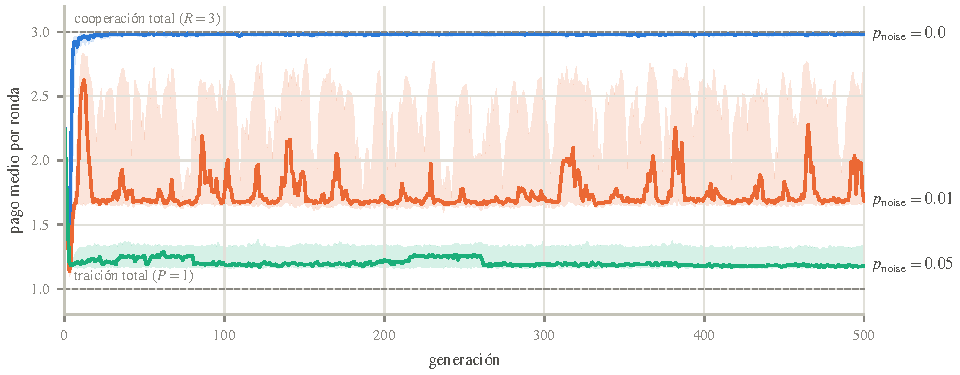
\includegraphics[width=\textwidth]{fig_pago_medio}
\caption{Pago medio por ronda de la población a lo largo de las generaciones: mediana (línea) y rango
intercuartílico (banda) de las 30 ejecuciones de cada nivel de ruido.}\label{fig:payoff}
\end{figure}

\begin{figure}[t]
\begin{minipage}[c]{0.47\textwidth}
\centering
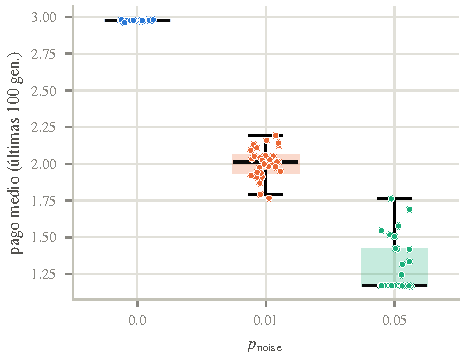
\includegraphics[width=\textwidth]{fig_pago_final}
\captionof{figure}{Variable respuesta (pago medio de las últimas 100 generaciones) de cada una de las 90
ejecuciones.}\label{fig:final}
\end{minipage}\hfill
\begin{minipage}[c]{0.5\textwidth}
\centering\small
\captionof{table}{Pago medio de las últimas 100 generaciones (30 ejecuciones por nivel): mediana con IC
bootstrap al 95\,\%, y comparaciones por pares ($p$ de Mann--Whitney corregido por Holm).}\label{tab:stats}
\begin{tabular}{@{}lcc@{}}
\toprule
$\pn$ & Mediana [IC 95\,\%] & Mín.--máx. \\
\midrule
0     & 2.978 [2.977, 2.979] & 2.963--2.983 \\
0.01  & 2.013 [1.976, 2.046] & 1.766--2.193 \\
0.05  & 1.171 [1.169, 1.325] & 1.166--1.761 \\
\midrule
Comparación & Dif.\ medianas [IC 95\,\%] & $\Atwelve$ \\
\midrule
0 vs 0.01    & $+0.966$ [$+0.932$, $+1.002$] & 1.00 \\
0 vs 0.05    & $+1.808$ [$+1.653$, $+1.809$] & 1.00 \\
0.01 vs 0.05 & $+0.842$ [$+0.679$, $+0.875$] & 1.00 \\
\bottomrule
\multicolumn{3}{@{}l}{\footnotesize En las tres comparaciones, $p_{\text{Holm}}=9\cdot10^{-11}$.}
\end{tabular}
\end{minipage}
\end{figure}

\begin{figure}[t]
\centering

\includegraphics[width=0.95\textwidth]{leyenda_estrategias}\\[2pt]
\threepanels{fig_frecuencias}
\caption{Frecuencia de las estrategias con nombre a lo largo de las generaciones (media de las 30
ejecuciones).}\label{fig:freq}
\end{figure}

\begin{figure}[t]
\centering

\includegraphics[width=0.95\textwidth]{leyenda_estrategias}\\[2pt]
\threepanels{fig_composicion}
\caption{Composición de cada ejecución, promediada en las últimas 100 generaciones. Cada barra es una
ejecución, ordenadas de menor a mayor pago final.}\label{fig:comp}
\end{figure}

\paragraph{Qué estrategias ganan.} Las Figuras~\ref{fig:freq} y \ref{fig:comp} muestran la composición
de la población. Decimos que una estrategia domina una ejecución si supera el 50\,\% de la población en
promedio en las últimas 100 generaciones.
\begin{itemize}
  \item \textbf{$\pn=0$:} TFT domina en 29 de 30 ejecuciones (mediana 78\,\%) y ocupa un régimen el 90\,\%
        del tiempo a partir de la generación 100. Casi todo el resto (OTRAS, 17\,\%) es el genoma \g{00100},
        que solo difiere de TFT en la respuesta a DD; entre cooperadores esa entrada no se usa nunca, así
        que es una variante neutra que deriva libremente. \textbf{H1 se confirma.}
  \item \textbf{$\pn=0.01$:} GRIM domina en 19 de 30 ejecuciones (mediana 53\,\%), seguida de TFT
        (13\,\%). PAVLOV no pasa de una mediana del 5\,\% y no domina en ninguna ejecución.
        \textbf{H2 se refuta.}
  \item \textbf{$\pn=0.05$:} ALLD domina en 19 ejecuciones (con un 95\,\% de la población) y GRIM en 9;
        en las 2 restantes conviven ambas. El pago cae a 1.17 en la mediana. \textbf{H3 se confirma},
        aunque la población no siempre termina en el mismo estado.
\end{itemize}

%=====================================================================
\section{Mecanismo}\label{sec:mec}
%=====================================================================
Para explicar estos resultados usamos la matriz de pagos esperados de las estrategias clásicas
(Figura~\ref{fig:matrix}), calculada con el mismo modelo exacto que la fitness. En una población grande
formada casi solo por una estrategia residente $X$, un mutante $Y$ puede invadirla si
$\pi(Y,X)>\pi(X,X)$, o si $\pi(Y,X)=\pi(X,X)$ y $\pi(Y,Y)>\pi(X,Y)$, donde $\pi(A,B)$ es el pago de $A$
contra $B$. La Tabla~\ref{tab:inv} aplica este criterio a cada nivel de ruido. Además, como la mutación
cambia un bit cada vez, miramos también la ventaja $\pi(Y,X)-\pi(X,X)$ de los 5 mutantes de un bit de cada
residente: si es casi nula, el mutante puede extenderse por deriva aunque no invada.

\begin{figure}[t]
\centering
\threepanels{fig_matriz}
\caption{Pago esperado por ronda de la estrategia de la fila contra la de la columna (150 rondas). Cuanto
más oscura la celda, mayor el pago.}\label{fig:matrix}
\end{figure}

\begin{table}[t]
\centering\small
\caption{Análisis de invasión: estrategias con nombre que pueden invadir una población de la residente.
«No invadible» indica que ninguna de las 32 estrategias de memoria~1 obtiene contra la residente un pago
igual o mayor que la propia residente.}\label{tab:inv}
\begin{tabular}{llll}
\toprule
Residente & $\pn=0$ & $\pn=0.01$ & $\pn=0.05$ \\
\midrule
ALLC   & ALLD, STFT & todas & todas \\
ALLD   & ---  & no invadible & no invadible \\
TFT    & ---  & ALLC & ALLC \\
PAVLOV & ALLD & ALLD, GRIM & ALLD, GRIM \\
GRIM   & ---  & no invadible & no invadible \\
STFT   & ALLC, TFT, PAVLOV, GRIM & ALLC, TFT, PAVLOV & ALLC, TFT, PAVLOV \\
\bottomrule
\end{tabular}
\end{table}

\paragraph{Sin ruido.} TFT, PAVLOV, GRIM y ALLC obtienen todas 3 entre sí, así que entre ellas la selección es
neutra. Lo que las distingue es cómo responden a los mutantes que traicionan, que el operador de mutación
genera constantemente. PAVLOV es invadible por ALLD: contra ALLD alterna C y D y solo obtiene 0.5, mientras
que TFT y GRIM obtienen 0.99. Los dos mutantes de un bit de TFT que traicionan (STFT \g{10101}, que
empieza con D, y \g{01101}, que traiciona tras CC) hacen que TFT entre en una alternancia de represalias que
le da un pago de 2.5, mientras que GRIM castiga para siempre y solo obtiene 1.02--1.03. Por eso GRIM domina
en las primeras generaciones, cuando todavía hay muchos traidores (pico inicial de la
Figura~\ref{fig:freq}a), pero TFT la desplaza en 25 de las 30 ejecuciones una vez que la población ya
coopera: frente a sus propios mutantes, TFT es la estrategia recíproca más rentable.

\paragraph{Con ruido moderado ($\pn=0.01$).} El ruido rompe el equilibrio de TFT: un error provoca una cadena
de represalias alternas, y el pago de TFT contra TFT cae a 2.52. Las variantes más indulgentes de TFT, como
ALLC o los mutantes de un bit \g{00001} y \g{00100}, que vuelven a cooperar tras una traición mutua,
obtienen más que TFT contra TFT (ventajas de $+0.43$ y $+0.20$) y la invaden. Una población así es
explotada a continuación por GRIM (4.00 contra ALLC) y ALLD (4.94). PAVLOV, que es la mejor contra sí
misma (2.95), es invadible por ALLD (2.99) y por GRIM (2.98), que explotan que PAVLOV vuelva a cooperar
tras una traición mutua. Por el contrario, GRIM no es invadible por \emph{ninguna} de las 32 estrategias de
memoria~1, aunque TFT queda casi empatada con ella (1.655 frente a 1.658). Así, GRIM es el atractor habitual
(ocupa un régimen el 50\,\% del tiempo), y su casi neutralidad respecto a TFT abre la puerta a ciclos: GRIM
deriva hacia TFT, las variantes indulgentes invaden a TFT y GRIM vuelve a explotarlas. En 22 de las 30
ejecuciones hay al menos un cambio de régimen, y en los periodos dominados por OTRAS las estrategias
principales son precisamente \g{00100}, \g{00001} y ALLC. La Figura~\ref{fig:cycles}b muestra estos
ciclos en una ejecución concreta; ellos explican los picos de cooperación de la Figura~\ref{fig:payoff} y por
qué el pago medio final (2.01) supera el de una población pura de GRIM (1.66).

\paragraph{Con ruido alto ($\pn=0.05$).} Los errores son tan frecuentes (en una pareja, uno cada 10 rondas
de media) que ninguna estrategia recíproca mantiene la cooperación: TFT contra TFT obtiene 2.30 y PAVLOV es
explotada por ALLD (2.93 frente a 2.78). Solo quedan dos estados no invadibles, ALLD y GRIM, y cada uno es
estable frente al otro: ALLD obtiene 1.18 contra GRIM, menos que GRIM contra GRIM (1.31), y GRIM obtiene 1.14
contra ALLD, menos que ALLD contra ALLD (1.15). Sin embargo, la población no se queda fija en uno de ellos:
pasa el 57\,\% del tiempo en un régimen de ALLD y el 34\,\% en uno de GRIM, y 18 de las 30 ejecuciones
cambian de régimen al menos una vez. La transición la permiten mutantes casi neutros: los mutantes de un bit
\g{10111} y \g{01111} de ALLD pierden solo 0.002 y 0.006 frente a ALLD, de modo que se extienden por deriva,
y \g{10111} (GRIM que empieza traicionando, el genoma más frecuente en las fases OTRAS) está a un solo bit
de GRIM. Así, la bimodalidad de la Figura~\ref{fig:comp}c es una fotografía de un proceso que alterna entre
dos estados de traición, ninguno de los cuales es cooperativo (Figura~\ref{fig:cycles}c).

\begin{figure}[t]
\centering

\includegraphics[width=0.95\textwidth]{leyenda_estrategias}\\[2pt]
\threepanels{fig_ejecucion}
\caption{Dinámica de una sola ejecución por nivel de ruido (ejecución 0). Con $\pn=0.01$ se observan ciclos
entre GRIM y variantes cooperativas; con $\pn=0.05$, una larga fase de ALLD seguida de un cambio a GRIM.}
\label{fig:cycles}
\end{figure}

\paragraph{¿Por qué no gana PAVLOV?} En el resultado clásico a favor de PAVLOV \cite{nowak1993}, obtenido con
estrategias estocásticas, PAVLOV solo se impone después de que estrategias tipo TFT hayan eliminado a los
traidores. Con estrategias deterministas de memoria~1, PAVLOV tiene una debilidad estructural: frente a un
traidor incondicional coopera una ronda de cada dos. Con nuestro operador de mutación, ALLD y GRIM reaparecen
continuamente y explotan esa debilidad antes de que PAVLOV pueda establecerse.

%=====================================================================
\section{Limitaciones}
%=====================================================================
\begin{itemize}
  \item \textbf{Solo memoria 1 y estrategias deterministas.} Estrategias más complejas (memoria~2,
        máquinas de estados) o estocásticas (\emph{generous TFT}) podrían sostener la cooperación con ruido.
        No estudiamos la extensión del enunciado; nuestras conclusiones se refieren al espacio de 32
        estrategias.
  \item \textbf{Un único conjunto de parámetros del GA.} La población de 100, $p_m=0.01$ y el torneo de 3
        fijan la intensidad de la deriva y de la selección. Como los cambios de régimen dependen de mutantes
        casi neutros, otra población u otra tasa de mutación cambiarían su frecuencia, y quizá la
        estabilidad de PAVLOV.
  \item \textbf{Sin autojuego.} Un individuo no juega contra sí mismo. Con población 100 el efecto es pequeño,
        pero no nulo.
  \item \textbf{El pago medio mezcla cooperación y ruido.} Con ruido alto, incluso ALLD contra ALLD obtiene
        más de 1, porque los errores producen cooperaciones involuntarias. Por eso complementamos el pago con
        la composición de la población.
  \item \textbf{Umbrales arbitrarios.} Las definiciones de dominancia y de régimen (50\,\% de la población,
        10 generaciones) son convenciones nuestras; los pagos y los tests no dependen de ellas.
  \item \textbf{Robustez.} En una comprobación adicional (10 ejecuciones por configuración,
        \texttt{report/robustness.py}) las conclusiones se mantienen con partidas de 1000 rondas
        (TFT domina en 10/10 sin ruido, GRIM en 6/10 con $\pn=0.01$ y ALLD en 6/10 con $\pn=0.05$) y con más
        ruido ($\pn=0.1$: ALLD en 8/10; $\pn=0.25$: ALLD en 10/10, con un pago de 1.70 que solo refleja el
        ruido). Sin embargo, no hemos explorado de forma sistemática otros niveles intermedios entre 0 y 0.01,
        donde debe estar la transición entre TFT y GRIM.
\end{itemize}

%=====================================================================
\section{Conclusiones}
%=====================================================================
En una población de estrategias de memoria~1 que evoluciona con un GA, la cooperación emerge y es estable
sin ruido, con TFT como estrategia dominante. Basta un 1\,\% de errores para perder un tercio del pago medio:
la población queda dominada por GRIM y atraviesa ciclos de cooperación y explotación. Con un 5\,\% la
cooperación colapsa y la población alterna entre dos estados de traición, ALLD y GRIM. La hipótesis se
cumple en los extremos, pero la estrategia indulgente PAVLOV no gana con ruido moderado, porque es explotable
por ALLD y GRIM, que no son invadibles por ninguna estrategia de memoria~1. El análisis de invasión sobre la
matriz de pagos esperados, completado con los mutantes casi neutros, explica tanto los ciclos como la
bimodalidad observados.

\paragraph{Reproducibilidad.} Todo el código, las semillas y las instrucciones están en el
\texttt{README.txt}: \texttt{python main.py} ejecuta el experimento y \texttt{python analysis.py} genera
todas las tablas (\texttt{results/summary.txt}) y las figuras de este informe.

\paragraph{Uso de herramientas de IA generativa.} Hemos utilizado Claude (Anthropic, modelo Claude Opus 5.5,
noviembre de 2026) como asistente para revisar el código inicial (detectó el problema de reutilizar una única
partida ruidosa por pareja), proponer y escribir el cálculo exacto del pago esperado, el script de análisis
estadístico y de figuras, y un primer borrador de este informe. Todos los resultados se han obtenido
ejecutando nuestro código, y hemos revisado, verificado y editado el texto final.

\small
\begin{thebibliography}{9}
\bibitem{arcuri2011} A.~Arcuri, L.~Briand. A practical guide for using statistical tests to assess randomized
  algorithms in software engineering. \emph{Proc.\ ICSE}, 1--10, 2011.
\bibitem{axelrod1987} R.~Axelrod. The evolution of strategies in the iterated prisoner's dilemma. In
  L.~Davis (ed.), \emph{Genetic Algorithms and Simulated Annealing}, Pitman, 1987.
\bibitem{efron1993} B.~Efron, R.~J.~Tibshirani. \emph{An Introduction to the Bootstrap}. Chapman \& Hall, 1993.
\bibitem{deap} F.-A.~Fortin, F.-M.~De~Rainville, M.-A.~Gardner, M.~Parizeau, C.~Gagné. DEAP: evolutionary
  algorithms made easy. \emph{Journal of Machine Learning Research} 13:2171--2175, 2012.
\bibitem{holm1979} S.~Holm. A simple sequentially rejective multiple test procedure. \emph{Scandinavian
  Journal of Statistics} 6(2):65--70, 1979.
\bibitem{nowak1993} M.~Nowak, K.~Sigmund. A strategy of win-stay, lose-shift that outperforms tit-for-tat in
  the Prisoner's Dilemma game. \emph{Nature} 364:56--58, 1993.
\bibitem{vargha2000} A.~Vargha, H.~D.~Delaney. A critique and improvement of the CL common language effect
  size statistics of McGraw and Wong. \emph{Journal of Educational and Behavioral Statistics} 25(2):101--132, 2000.
\bibitem{wu1995} J.~Wu, R.~Axelrod. How to cope with noise in the iterated prisoner's dilemma. \emph{Journal
  of Conflict Resolution} 39(1):183--189, 1995.
\end{thebibliography}

\end{document}
